\subsubsection{Assigning Codes:}

When the coding tree has been created, we need to used to create a new dictionary that will store the code of each {\itshape symbol}. To make this, we need to set a marker in each leaf of the tree, all the left and right leafs will have the labels " 0" and "1" respectively, so then, each {\itshape symbol} will have as code the string of "0's" ans "1's" that need to traversal to reach it as we can see in Figure 3.3.0: \hfill \break

\begin{figure}[H]
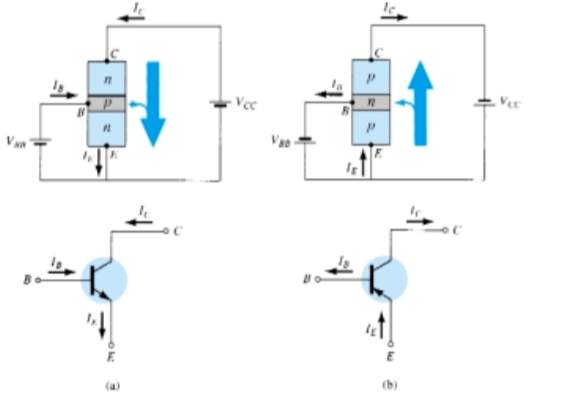
\includegraphics[height = 7cm, width = 16.5cm]{5.png}
\centering \linebreak \linebreak Figure 3.3.0: Binary codes for each symbol.
\end{figure} \hfill \break

To make this on our code, we will use DFS ( Depth-First Search ) on the tree by generating the codes as we go down on the branches. \hfill \break

\begin{lstlisting}
def setCodes ( self ):
        # Depth-First Search stack.
        searchStack = [ ]
        searchStack.append ( self.tree + ( "", ) )
        while ( len ( searchStack ) > 0 ):
            element = searchStack.pop ( )
            if ( type ( element [ 2 ] ) == list ):
                # The node it's not a leaf.
                searchStack.append ( element [ 2 ] [ 1 ] + ( element [ -1 ] + "1", ) )
                searchStack.append ( element [ 2 ] [ 0 ] + ( element [ -1 ] + "0", ) )
            else:
                # The node it's a leaf.
                code = element [ -1 ]
                self.codes [ element [ 2 ] ] = code
            pass
\end{lstlisting} \hfill \break

The code works as follows, in line 3 we declare a stack to make the DFS, in line 4 we append to the structure the tree and its "prefix" or label that we will set for this leaf, because it is the root will set the marker "". Then from lines 5 - 15 there is a {\bfseries while} loop. In line 6 we will pop the last element in the stack ( FIFO ), in case that the element popped it's of {\itshape type} list it means that it's a sub-tree and has two children ( left and right nodes ), in lines 9 - 10 we will add the respectively labels to each leaf and continue with the iterations. In the other case we will ask for the respective code of that leaf in line 13 for later appended to the codes dictionary as we can see in line 14. Finally, the codes dictionary should look as:

\begin{center}
self.codes = $\lbrace$ "a": 0, "b": 10, "c": 111, "END": 110 $\rbrace$
\end{center}

\pagebreak
